\section{Floquet exponents and {\cLvs} by Periodic Schur Decomposition }
\subsection{Introduction to Periodic Schur Decomposition}

	\paragraph{Real Schur Decomposition}
		For an arbitrary real $N\times N$ matrix $A$, the information about its eigenvalues and eigenvectors
		are stored in its \textit{real Schur decomposition}:
		\[
			A=Q^{T}TQ
		\]
		where $Q$ is a real orthogonal matrix and $T$ is a quasi-upper triangular matrix with real
		eigenvalues on the diagonal and complex eigenvalue pairs in the $2\times 2$ blocks on the
		diagonal. The Schur decomposition represents the rotation of matrix $A$ in $N$ dimensions,
		so $A$ and $T$ have the same set of eigenvalues and the relation between their eigenvectors
		is simple:
		\begin{center}
		if $Tx=\lambda x$, then $A(Q^{T}x)=\lambda (Q^{T}x)$.
		\end{center}
		Therefore, the problem of
		calculating eigenvalues and eigenvectors of matrix $A$ is transformed to the same problem of
		a much simpler matrix $T$.

		Matrix $T$ has quasi-upper triangular form, so the eigenvalues are just the diagonal elements or
		the complex eigenvalues of the $2\times 2$ matrix on the diagonal. At the same time, if we align
		its eigenvectors into a $N\times N$ matrix $V=[v_{1}, v_{2},\cdots,v_{N}]$, then the eigenvector
		matrix $V$ is quasi-upper triangular too! This idea is obvious if you use Gaussian Elimination
		method to find the eigenvectors of quasi-upper triangular matrix $T$. I cannot address the
		importance of this observation more because it is the basis of calculating {\cLvs}
		by Periodic Schur Decomposition.

	\paragraph{How about a product of matrices: $M=M_{2}M_{1}$ }

		For \KSe, we already have a large number of \rpo s, which are
useful for us 		to analyze the dimension of the attractor. For this
purpose, the eigenvalues (Floquet multipliers) 		and the eigenvectors
(Floquet vectors) of the Jacobian matrix for a relative periodic orbit 		
are needed.

		However, the usual way is not suitable to the problem here because the Floquet multipliers spectrum has
		a large span which is beyond the domain of double precision number. There is also a danger that
		the elements of Jacobian matrix will overflow or underflow when you evolve the system for
		a relative long time. In this sense, the Jacobin matrix should not be explicitly expressed, but the
		question is how we can get the eigenvalues and eigenvectors of a matrix which is not written down.
		To bypass this problem, we can use the factorization property of Jacobian matrix:
		\begin{equation}
			J^{t-t_{0}}(x_{0},t_{0})=J^{t-t_{1}}(x(t_{1}),t_{1})J^{t_{1}-t_{0}}(x(t_{0}),t_{0})
		\label{eq:xjacobian}
		\end{equation}
		where $x(t_{1})=f(x(t_{0}), t_{1}-t_{0})$ is the orbit point after evolving the system from point
		$x(t_{0})$ for a period $t_{1}-t_{0}$. \refeq{eq:xjacobian} basically states that the Jacobian
		matrix associated with a long orbit can be factorized as the product of Jacobian matrices which
		are associated with short segments of this orbit. In this way, we can express the Jacobian matrix
		as a product of many matrices with the same dimension. It depends on the dynamics of the system
		to determine how many matrices we need to factorize it to, and the least criteria is that the elements
		of these matrices should spread in a relatively small range.

		Now we come to the core problem: how to get the eigenvalues and eigenvectors of a product of matrices?
		\begin{per_schur}
			\textbf{Periodic Schur Decomposition : }
			Let $M_{j}\in \mathbb{R}^{N\times N}$, $j=1,2,\cdots,m$. Then there exits orthogonal matrices
			$Q_{j}\in \mathbb{R}^{N\times N}$ such that
			\begin{center}
				$R_{1}=Q^{T}_{1}M_{1}Q_{m}$\\
				$R_{2}=Q^{T}_{2}M_{2}Q_{1}$\\
				$R_{3}=Q^{T}_{3}M_{3}Q_{2}$\\
				$\cdots$\\
				$R_{m}=Q^{T}_{m}M_{m}Q_{m-1}$\\
			\end{center}
			where, $R_{1},R_{2},\cdots, R_{m-1}$ are upper-triangular matrices, and $R_{m}$ is a quasi-upper
			triangular matrix with real eigenvalues on the diagonal and complex eigenvalue pairs in
			the $2\times 2$ blocks on the diagonal.

		\end{per_schur}
		The proof of this theorem is given in paper \rf{Bojanczyk92theperiodic,Lust01}.
		Let $M=M_{m}\cdots M_{2}M_{1}$ and $R=R_{m}\cdots R_{2}R_{1}$, and then $R=Q^{T}_{m}MQ_{m}$, which is
		the real Schur decomposition of matrix $M$, so the problem of calculating eigenvalues and eigenvectors
		of matrix product $M$ is transformed to the same problem of matrix product $R$. Since matrix $R$ is a product
		of $m-1$ upper-triangular matrices and 1 quasi-upper triangular matrix, $R$ is quasi-upper triangular too.
		Its diagonal element (or $2\times 2$ block) is just the product of the diagonal elements (or $2\times 2$ blocks) of
		$R_{m},\cdots, R_{2},R_{1}$ at the same position.

		In application, we choose to add the logarithm of the diagonal elements to avoid data overflow or downflow; in the
		meantime, the eigenvectors of matrix $M$ are obtained from  eigenvectors of $R$ rotated by the orthogonal matrix
		$Q_{m}$.
		
\subsection{An implementation of Periodic Schur Decomposition }
\label{sect:PSDimpl1}
	The process of conducting \psd\ is described in paper \rf{Bojanczyk92theperiodic,Lust01}, and the pseudo code is provided
	in this \HREF{https://perswww.kuleuven.be/~u0006235/ACADEMIC/r_psSchur.html}{website}, which also gives the Fortran
	implementation. I implement the algorithm in Matlab and the code is saved in the folder
	\texttt{siminos/xiong/matlab/periodic\_schur}, which is not the ultimate version.
	
	\subsubsection{Algorithm}
		\begin{figure}[h]
			\centering
			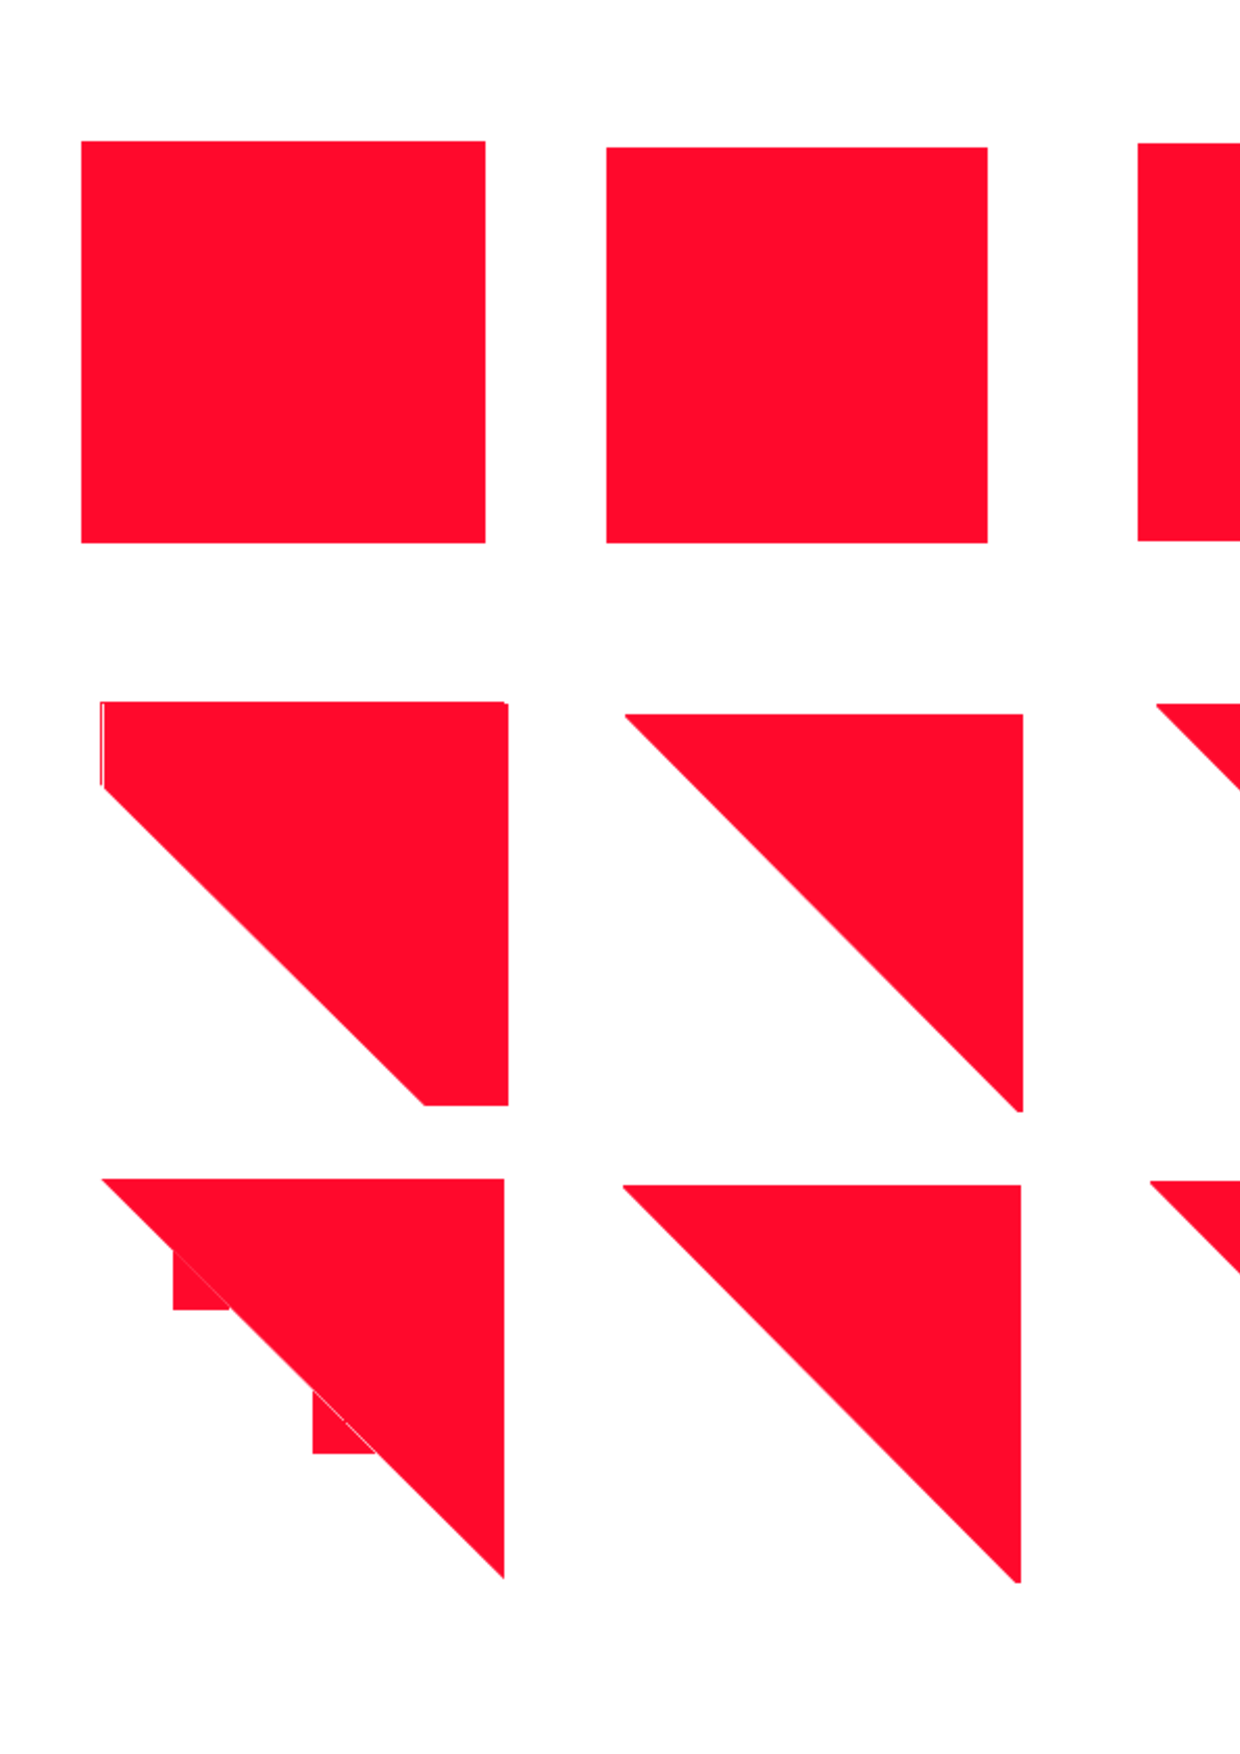
\includegraphics[width=0.8\textwidth]{per_schur_algorithm.pdf}
			\caption{demonstration of the process of conducting \psd\ .}
			\label{fig:per_schur_algorithm}
		\end{figure}
		There are two stages in conducting \psd\ .
		\begin{itemize}
			\item stage 1: transformation to  Hessenberg-triangular from
			\item stage 2: transformation to  quasi-upper triangular form
		\end{itemize}
		These two stages are demonstrated in Fig \ref{fig:per_schur_algorithm}. In this example, the number of matrices
		is set to 3 : $M=M_{3}M_{2}M_{1}$. The first row shows these three square matrices $M_{3},M_{2},M_{1}$ and
		red color means the elements there are nonzero numbers; while white places are all zeros. Initially, these
		three matrices are all dense.
		
		\paragraph{Stage 1}
		The transition from first row to the second row in \ref{fig:per_schur_algorithm} is the first stage.
		\begin{itemize}
			\item input: dense matrices $M_{3},M_{2},M_{1}$.
			\item output: upper-triangular matrices  $H_{2},H_{1}$ and upper-hessenberg matrix $H_{3}$.\\
					orthogonal matrices $Q_{3},Q_{2},Q_{1}$, such that $Q^{T}_{i}M_{i}Q_{i-1}=H_{i}$,
					$Q_{0}=Q_{3}$.
		\end{itemize}
		This transition is realized by a set of consecutive Householder reflections, whose details are described in
		\textit{siminos/xiong/matlab/periodic\_schur/algorithms.pdf}. The required number of Householder reflections
		is $O(mN)$, where $m$ is the number of matrices ($m=3$ in this example) and $N$ is the matrix dimension,
		therefore the number of total operations is $O(mN^{3})$, which is every cheap.

		The relative error associated with the first stage is small by the result of my testing. The above figure in
		Fig \ref{fig:err_hess_trian} showed that the absolute error is around $10^{-14}$ for 3000 matrices of
		dimension $30\times 30$.
		\begin{figure}[h]
			\centering
			\includegraphics[width=0.7\textwidth]{err_hess_trian.pdf}
			\caption{absolute error associated with two stages, which are tested on 3000 random matrices of
			dimension $30\times 30$. The y-axis is the norm of columns of error matrices
			$E_{i}=Q^{T}_{i}M_{i}Q_{i-1}-H_{i}$ for stage 1 and $E_{i}=\hat{Q}^{T}_{i}H_{i}\hat{Q}_{i-1}=R_{i}$
			for stage 2, so there are total $3000*30=90000$ points. The x-axis is the indices
			of these columns.
			}
			\label{fig:err_hess_trian}
		\end{figure}

		\paragraph{Stage 2}
		The transition from second row to the third row in \ref{fig:per_schur_algorithm} is the second stage.
		\begin{itemize}
			\item input: upper-triangular matrices $H_{2},H_{1}$ and upper-hessenberg matrix $H_{3}$.
			\item output: upper-triangular matrices $R_{2}, R_{1}$ and quasi-upper triangular matrix $R_{3}$.\\
					orthogonal matrices $\hat{Q}_{3},\hat{Q}_{2},\hat{Q}_{1}$, such that
					$\hat{Q}^{T}_{i}H_{i}\hat{Q}_{i-1}=R_{i}$,
					$\hat{Q}_{0}=\hat{Q}_{3}$.
		\end{itemize}
		Stage 2 is called ``periodic QR'' step in paper \rf{Bojanczyk92theperiodic} because the basic process
		in this stage is conducting QR iteration periodically, which is an extension of ``Francis's Algorithm''
		in the singe matrix case. The convergence of this stage is guaranteed by
		\HREF{http://people.inf.ethz.ch/arbenz/ewp/Lnotes/chapter3.pdf}{``Implicit Q theorem''}.
		For each iteration, the number of each Givens rotation is $O(mN)$, and the cost of Givens rotation
		is roughly $O(N)$, so the cost of each iteration is $O(mN^{2})$, which seems very cheap at the first
		glance. However,
		the converging rate of this stage is a not that optimistic, at least for \KS\ system.

		Paper \rf{Bojanczyk92theperiodic} introduces two different shift methods in this stage so as to get a
		better converging rates: \textit{single-shift step} and \textit{double-shift step}. But for me,
		choosing the appropriate shift is just like black magic and all my trials just backfire, so I choose
		not to use shift at all in my code. Maybe I should have put enough effort in this stage.
		If someone can find a reliable method to select the shift, hope you can tell me.
			
		Again, the numerical error associated with stage 2 is small as shown in Fig \ref{fig:err_hess_trian},
		which is the result of a test on a product of 3000 matrices.

		\paragraph{Note} The original algorithm consists of 4 stages, but I only introduce 2 of them because these
		2 stages are enough for \KS\ system. The other two stages are \textit{Deflation} and \textit{Eigenvalues
		reodering}. When the matrix product is singular, we need to get rid of zero elements on the diagonal of these
		upper-triangular matrices, where \textit{Deflation} is used. In this sense, \psd\ can be used for singular
		matrix too, but I don't think Jacobian matrix of \KSe\ is singular. At the same time, the Floquet multipliers
	 	are ordered by themselves for \KS\ system, so there is no need to reorder the eigenvalues.

	\subsubsection{Eigenvalues}
		Assume that stage 2 is accomplished and we have $m$ matrices: $M_{1},M_{2},\cdots,M_{m}$,
		the first $m-1$ of which are upper-triangular matrices and the last one is quasi-upper triangular matrix.
		It is time to calculate the eigenvalues right now.

		The process is quite simple. If the $i_{th}$ eigenvalue is real, then it is just the product of all the $i_{th}$
		diagonal elements of matrices $M_{1},M_{2},\cdots,M_{m}$. In practice, the logarithm of these numbers is added
		to overcome overflow or downflow. If the $i_{th}$ and $(i+1)_{th}>$ eigenvalues are complex conjugate pairs,
		we just need to multiply all the $2\times 2$ matrices at position $(i,i+1)$ on the diagonal, and the two
		eigenvalues of this product are what we need. There is no danger of overflow because all these $2\times 2$
		matrices are in the same position and their elements should have similar order of magnitude, which is at least
		true for \KS\ system.

	\subsubsection{Eigenvectors}
		My method to calculate eigenvectors is based on power iteration and the prerequisite is that all the eigenvalues
		are ordered in ascending or descending order by their magnitude. This method cannot deal with degenerate case, but
		it is capable to get the complex eigenvector pair.

		Suppose the \psd\ of $J=M_{m}\cdots M_{2}M_{1}$ is $Q^{T}_{m}JQ_{m}=R_{m}\cdots R_{2}R_{1}$, where $Q_{m}$ is an
		orthogonal matrix, $R_{m-1},\cdots, R_{2},R_{1}$ are upper-triangular matrices and $R_{m}$ is quasi-upper triangular.
		We only need to calculate eigenvectors $v_{i}, i=1,2\cdots, N$ of matrix $R=R_{m}\cdots R_{2}R_{1}$
		because eigenvectors of $J$ are related to $v_{i}$ by $Q_{m}$. The basic idea is that \textbf{the eigenvector matrix
		[$v_{1}$,$v_{2}$,$\cdots$,$v_{N}$] of a quasi-uppper triangular matrix is quasi-upper triangular too}.
		
		\paragraph{Real eigenvectors}
			If the $i_{th}$ eigenvector is real, then it has the form
			\begin{center}
				$v_{i}=(a_{1},a_{2},\cdots,a_{i},0,\cdots, 0)^{T}$.
			\end{center}
			First, Let's assume that all the eigenvalues are ordered ascend:
			$|\ExpaEig_{1}|<|\ExpaEig_{2}|<\cdots<|\ExpaEig_{N}|$.
			An arbitrary vector whose first $i$ elements are nonzero $x=(b_{1},b_{2},\cdots,b_{i},0,\cdots, 0)^{T}$
			is a linear combination of the first $i$ eigenvectors.
			\begin{center}
				$x=\alpha_{1}v_{1}+\alpha_{2}v_{2}+\cdots+\alpha_{i}v_{i}$.
			\end{center}
			Use it as the initial guess for the power iteration and after $k$ iterations:	
			\[
			R^{k}x=\ExpaEig_{i}^{k}(\alpha_{1}\frac{\ExpaEig_{1}^{k}}{\ExpaEig_{i}^{k}}v_{1}
					+\alpha_{2}\frac{\ExpaEig_{2}^{k}}{\ExpaEig_{i}^{k}}v_{2}
					+\cdots
					+\alpha_{i}v_{i})
			\]
			It is clear to see that if this vector is normalized after each iteration, then it will converge to the
			$i_{th}$ eigenvector of $R$:
			\[
			\lim_{k\to \infty} \frac{R^{k}x}{|R^{k}x|}=v_{i}
			\]

			Second, Let's assume that all the eigenvalues are ordered descend:
			$|\ExpaEig_{1}|>|\ExpaEig_{2}|>\cdots>|\ExpaEig_{N}|$.
			Since $Rv_{i}=\ExpaEig_{i}v_{i}$, then $R^{-1}v_{i}=\ExpaEig_{i}^{-1}v_{i}$. $R$ and $R^{-1}$ have the
			same set of eigenvectors with reciprocal eigenvalues, so the eigenvalues of
			$R^{-1}=R_{1}^{-1}R_{2}^{-1}\cdots R_{N}^{-1}$ are ordered ascend. We go back to the first case!
			I use this method to get {\cLvs} for \KS\ system. Note that this process is numerically
			practicable because each $R_{i}$ is well conditioned if the time step is small enough.

			What if the eigenvalues are not ordered ascend or descend ? I just omit this situation because the
			eigenvalues for \KS\ system are ordered descend, but I think you need to reorder eigenvalues in the
			\psd\ .

		\paragraph{Complex eigenvector pair}
			The eigenvectors corresponding to the complex eigenvalues are complex and they appear as pairs.
			Power iteration will fail in this case because now two eigenvalues have the same magnitude:
			$\ExpaEig_{i}$ and $\ExpaEig_{i}^{*}$. If you start the power iteration with a real vector, then
			you will find that it is stretching or contracting in an oscillating style.
			
			We can introduce complex shift to resolve this problem. Let the $i_{th}$ eigenvalue to be
			$\ExpaEig_{i}=a+ib$, where $b>0$, then the $(i+1)_{th}$ eigenvalue is $\ExpaEig_{i+1}=a-ib$. It is obvious
			that $R+is\mathbf{I}$ and $R$ have the same eigenvectors, where $s$ is an arbitrary real number.
			\begin{align*}	
			(R+is\mathbf{I})v_{i} & =[a+i(b+s)]v_{i}\\
			(R+is\mathbf{I})v_{i+1} & =[a+i(-b+s)]v_{i+1}
			\end{align*}	
			So $R+is\mathbf{I}$ can be used in the power iteration instead of $R$. If $s>0$, it will converge to $v_{i}$
			since $b>0$. If $s<0$, it will converge to $v_{i+1}$.

			One point should be stressed. If $v_{i}$ is the eigenvector corresponding to $\ExpaEig_{i}=a+ib$, then
			$e^{i\theta}v_{i}$ is also an eigenvector corresponding to the same eigenvalue, where $\theta$ is an
			arbitrary real number. In this sense, complex eigenvector is not defined uniquely. In my code, I just force
			the first element of complex eigenvector to be real, and then this vector is determined precisely.
			
			The choice of shift $s$ is based on the criteria that it should split the magnitudes of these two eigenvalues
			as large as possible so that the converging process is fast.

		



\subsection{Floquet exponents and {\cLvs}}

	Now we apply \psd\ to \KS\ system. In this part, I will exhibit the Floquet
	exponents and  the {\cLvs} for two pre-\po s of
	\KSe: \cycle{ppo1} and \cycle{ppo9} in Ruslan's data file:
\\
	\texttt{siminos/matlab/ruslan/ks22f90h25t100.mat}. $\cycle{ppo1}$ has a prime
	period $\period{ppo1}=10.25\cdots$ and $\cycle{ppo9}$ has a prime period $\period{p9}=41.55\cdots$.
	\refFig{fig:ppo19_phase123} shows the configuration of these two orbits evolved
	for their prime periods respectively, and it shows that the  full period is twice
	the prime period in both cases.

	The group operation that transforms $x(0)$ to
	$x(t_{p})$ is reflection: $Ru(x)=-u(-x)$, which is
	\begin{align*}	
	R \, \Re a_{i} & =-\Re a_{i} \qquad i \mbox{odd}\\
	R \, \Im a_{i} & =\Im a_{i}  \qquad i \mbox{even}
	\end{align*}
	in Fourier coefficient space. Therefore, the group representation in both cases is
	\[
	g_{p}=diag(-1,1,-1,1,\cdots)
	\]
	\begin{figure}%[h]
	\centering
		\includegraphics[width=0.8\textwidth]{ppo19_phase123.pdf}
		\caption{Demonstration of the evolution of the first
		three Fourier coefficients for pre-\po s \cycle{ppo1} and \cycle{ppo9}.
		}
		\label{fig:ppo19_phase123}
	\end{figure}
	
	\paragraph{Relation between $g_{p}J^{\period{p}}$ and $J^{2\period{p}}$}
		I will give my result for Floquet exponents and
		{\cLvs} by two different matrices: $g_{p}J^{\period{p}}$ and
		$J^{2\period{p}}$. The former one is the definition of Jacobian matrix for
		relative periodic orbits, while the latter is just the Jacobian matrix for
		the full period, so we need to know their relation first.
		
		The orbits $\cycle{ppo1}$ and $\cycle{ppo9}$ are equivariant under group operation
		$g_{p}$:
		\[
		g_{p}f^{\period{p}}(x(0))=f^{\period{p}}(g_{p}x(0))
		\]
		where $f^{t}(x)$ is the flow equation of \KS\ system. Take the derivative of $x(0)$
		at both side and use the definition of Jacobian matrix
		$J^{t}(x)=\frac{\partial f^{t}(x)}{\partial x}$ , we have
		\[
		g_{p}J^{\period{p}}(x(0))=J^{\period{p}}(g_{p}x(0))g_{p}
		\]
		Therefore,
		\begin{align*}
			 J^{2\period{p}}(x(0)) & =J^{\period{p}}(x(\period{p}))J^{\period{p}}(x(0))	\\	
			& =J^{\period{p}}(g_{p}x(0))J^{\period{p}}(x(0))\\
			& =J^{\period{p}}(g_{p}x(0))g_{p}g_{p}J^{\period{p}}(x(0))\\
			& =g_{p}J^{\period{p}}(x(0))g_{p}J^{\period{p}}(x(0))
			  =(g_{p}J^{\period{p}}(x(0)))^{2}\,.
		\end{align*}
		During the process, I used the identity $g_{p}^{2}=\mathbb{I}$
        for reflection symmetry group $\Dn{2}$. Define
		\begin{equation}
		J_{p}=g_{p}J^{\period{p}}
		\label{eq:relative_jacobian}
		\end{equation}
		so we have relation:
		\begin{equation}
			J^{2\period{p}}=(J_{p})^{2}
		\label{eq:relationofjpj2t}
		\end{equation}
		Therefore, these two matrices have the same eigenvectors and the
eigenvalues of $J^{2\period{p}}$ are just square of the
corresponding ones of $J_{p}$, which means all the real eigenvalues of
$J^{2\period{p}}$ are positive. I will check this relation in the
following sections.
            \PC{Eventually, you want to make this argument totally
            general and simpler: I think you only need to know that the symmetry
            group actions commute with the dynamics, and for pre-periodic
            prime orbits (in case of discrete symmetries) the identity
            $g_{p}^{m}=\mathbb{I}$. How about reading
            \HREF{http://www.streamsound.dk/book1/chaos/chaos.html\#184/z}
            {ChaosBook} :)
                }
		
	\subsubsection{Floquet exponents}
		Floquet multipliers $\ExpaEig_{i}$ are defined as the eigenvalues of Jacobian matrix for periodic
		orbit. For relative periodic orbits, Jacobian is defined in \eqref{eq:relative_jacobian}.
		Floquet exponents $\lambda_{i}$ are defined as
        $\ExpaEig_{i}=\exp\left(\period{p}\Lyap_{i}\right)$. If Floquet exponent
        is complex, then it is written as
        $\Lyap_{i}=\eigRe[i]+i\eigIm[i]$.
		\refTab{tab:FloqExpPPO1} contains the Floquet exponents I got for the orbit $\cycle{ppo1}$ with
		respect to two different methods: one evolves the system for $\period{p1}$ and conducts group transformation;
		the other just evolves the system for $2\period{p1}$.
            \PC{
            Why plot $e^{i\period{p}\eigIm[i]}$? The $\pm$ sign is the
            character of $g_{p}$, and you want to show that the two
            $\eigIm[i]$ are the same, not compare $\cos \eigRe[i]$ with
            $\cos 2\eigRe[i]$? That serves no purpose. \eigRe[i] and \eigIm[i]
            are \emph{rates per unit time}, they are the same for any repeat of the
            the prime orbit.
                }
		
\input ../xiong/tables/FloqExpPPO1
		
\refTab{tab:FloqExpPPO1} shows that there are two complex eigen-pairs:
$(1,2)$ and $(6,7)$. All the other exponents are real. There are several
points needed to be stressed.

		\paragraph{Error analysis of the result}
		From previous analysis and \eqref{eq:relationofjpj2t}, we know that the first column should be the same
		with the third column in \reftab{tab:FloqExpPPO1}, and the square of second column should
		coincide with the fourth column. The observation is that these two relation is confirmed in a certain
		degree, but the accuracy is only about $10^{-4}$. It looks pessimistic
		to get such a large error, but we should locate the sources of this error before casting some doubt on
		\psd\ .
		
		The error has two sources:
		the \KSe\ solver and the \psd\ algorithm described here.
		Theoretically, the orbit transformed by $g_{p}$ after evolving for $\period{p}$ should coincide with the orbit
		after evolving for $2\period{p}$. But I find that
		\[
		|g_{p}f^{\period{p}}(x(0))- f^{2\period{p}}(x(0))|=2.627440335452566e-04		
        \,,
        \]
which has just the same magnitude of the total error. Therefore, there is
a great likelihood that the total error mainly comes from \KSe\ solver.

		On the other hand, we can check the error associated with \psd\ separately.
		\begin{figure}[h]
			\centering
			\includegraphics[width=0.8\textwidth]{err_psd.pdf}
			\caption{Difference of Floquet exponents. Red line: the prime orbit is partitioned into 500 and
			1000 segments respectively. Evolve the system for $\period{p}$
			and calculate the corresponding Floquet exponents. The red line shows the difference of
			their magnitudes pair wisely. Green line: the full orbit is partitioned into 1000 and 2000
			segments respectively and evolve the system for $2\period{p}$.}
			\label{fig:err_psd}
		\end{figure}
		Fig \ref{fig:err_psd} clearly shows that the error originated from \psd\ is around $10^{-13}$.We
		are relieved now!

		\paragraph{Observations}

		\begin{figure}[h]
			\centering
			\includegraphics[width=0.8\textwidth]{floquet_spectrum19.pdf}
			\caption{ Floquet exponent spectrum for prime orbit $\cycle{ppo1}$ and $\cycle{ppo9}$.
			The inner graph is the magnification of the first 8 exponents. For these complex exponents,
			just take $\mu_{i}$ as defined before.
			}
			\label{fig:floquet_spectrum19}
		\end{figure}
		
			Table \ref{tab:FloqExpPPO1} tells us that Floquet exponent could be negative, which
			means the corresponding eigenvector reverses its direction after one prime period. Also it
			could be complex pair, which means that any vector in its eigenspace  will rotate inside this
			subspace.

			\refFig{fig:floquet_spectrum19} shows $\mu_{i}$ (the first column in table
			\ref{tab:FloqExpPPO1}) for prime orbit $\cycle{ppo1}$ and $\cycle{ppo9}$. $9_{th}$ to
			$30_{th}$ floquet exponents are almost the same for both orbits (proportional to the
			forth order of Fourier mode index). $(1,2)$ and $(6,7)$ are two pairs of complex
			Floquet exponents for $\cycle{ppo1}$; while orbit $\cycle{ppo9}$ has only one complex pair: $(7,8)$.





	\subsubsection{\cLvs}
	
	\paragraph{Configuration}
		\refFig{fig:ppo1ev_low} and \ref{fig:ppo1ev_high} show the configuration of some {\cLvs} for \KS\ system,
		which clearly shows that the {\cLvs} corresponding to high Fourier modes are just localized around
		its mode index; while the first few {\cLvs} spread among first few indices.
		\begin{figure}[h]
		\centering
			\includegraphics[width=0.9\textwidth]{ppo1ev_low.pdf}
			\caption{The $1_{st}$ and $8_{th}$ \cLvs for the \cycle{ppo1} orbit ($\period{P}=10.25\cdots$).
			X-axis is the index of the elements of a vector.
			}
			\label{fig:ppo1ev_low}
		\end{figure}

		\begin{figure}[h]
		\centering
			\includegraphics[width=0.9\textwidth]{ppo1ev_high.pdf}
			\caption{The $20_{th}$, $25_{th}$ and $30_{th}$ \cLvs for the \cycle{ppo1} orbit ($\period{P}=10.25\cdots$).
			X-axis is the index of the elements of a vector.
			}
			\label{fig:ppo1ev_high}
		\end{figure}

	\paragraph{Expansion/contraction rate of \cLvs}
		When {\cLvs} evolve along the orbit, their expansion/contraction rate is recorded. \refFig{fig:ppo1rate}
		shows that the $8_{th}$ vector behaves well along the orbit, and the contraction rate is obviously periodic.
		While, vector $v_{10}$ is contaminated by other more expanding vectors after a short time. \Xiongedit{Kazz: This means that your choice of the time step and/or the interval between two Gram-Schmidt orthonormalization is not short enough. You have to set them to be, at the longest, $\mathcal{O}(|\lambda|_{\rm max}^{-1})$, where $|\lambda|_{\rm max}$ is the largest absolute value of the Lyapunov exponent you are interested in (here it is set by the most negative Lyapunov exponent).}
		\begin{figure}[h]
		\centering
			\includegraphics[width=1.0\textwidth]{ppo1rate.pdf}
			\caption{ The expansion/contraction rate of several {\cLvs} for orbit \cycle{ppo1}. The x-axis is time and
			time step is $\period{p}/1000$. Y-axis is logarithm the expansion rate of these vectors along the orbit. The total
			time is $2\period{p}$.
			}
			\label{fig:ppo1rate}
		\end{figure}
	
	\paragraph{Vector field }
		For periodic orbit, the velocity coincides with the \cLv\ that corresponds to
		a marginal Floquet multiplier. \refTab{tab:FloqExpPPO1} shows there are two
		marginal Floquet multipliers for orbit \cycle{ppo1}: $3_{rd}$ and $4_{th}$. The evolution of the third covariant
		vector is shown in \refFig{fig:ppo1vectorfield123}, from which we can conclude this
		{\cLv} is just the local velocity along the orbit.
		
		The same goes for orbit \cycle{ppo9}. In this case, the second \cLv\ represents the local
		velocity along the orbit, which is demonstrated in \refFig{fig:ppo9vectorfield123}.
		\begin{figure}[h]
		\centering
			\includegraphics[width=1.0\textwidth]{ppo1vectorfield123.pdf}
			\caption{The orbit \cycle{ppo1} and the evolution of the third \cLv. X, Y and Z axis
			are the first, second and third element of the state vector.
			}
			\label{fig:ppo1vectorfield123}
		\end{figure}

		\begin{figure}[h]
		\centering
			\includegraphics[width=1.0\textwidth]{ppo9vectorfield_mlab.png}
			\caption{The orbit \cycle{ppo9} and the evolution of the second \cLv\. X, Y and Z axis
			are the first, second and third element of the state vector.
			}
			\label{fig:ppo9vectorfield123}
		\end{figure}

\begin{figure}[h]
  \centering
  \includegraphics[width=1.0\textwidth]{ppo1FloquetVector}
  \caption{The 1st, 2nd, 25th and 26th Floquet vectors of
    preperiodic orbit \cycle{ppo1} with truncation number
    $N=32$. The x-axis is the Fourier mode
    indices. Note Matlab \texttt{fft()} orders wave numbers as
    $k=0,1,2,\cdots,N-1$ which is mapped to
    $k=0,1,\cdots,N/2-1,N/2,-N/2+1,\cdots,-1$ here. Also,
    mode $a_0$ and $a_{N/2}$ are ignored here because they are set to
    zero at the very beginning.
    Each Fourier mode
    has a real and imaginary part: $a_k=b_k+ic_k$. Floquet vectors
    are calculated in space $[b_1, c_1,\cdots,b_{N/2-1},c_{N/2-1}]$
    first and then their modulus at each mode is obtained:
    $|a_{k}|=|b_k+ic_k|$. Also note only half of them are needed since
    $a_{-k}=b_{k}-ic_{k}$. If Floquet vector is real ($v_{25}$, $v_{26}$),
    then $|a_{k}|=|a_{-k}|$, that is, they are self-dual under reflection
    along $x=0$.
    If Floquet vectors form complex conjugate pair ($v_1$, $v_2$), then
    there are relations
    $b^{(1)}_{k}=(b^{(2)}_{k})^{*}$ and $c^{(1)}_{k}=(c^{(2)}_{k})^{*}$,
    so
    $
    |a_{k}^{(1)}|=|b_k^{(1)}+ic_{k}^{(1)}|=|(b_{k}^{(1)})^{*}-i(c_{k}^{(1)})^{*}|
    =|b_k^{(2)}-ic_{k}^{(2)}|
    =|a_{-k}^{(2)}|
    \,.
    $
    Therefore, $v_1$ is dual to $v_2$ under reflection in this figure.
    In summary, actually, only half of the this figure is enough.
    This figure is different from \reffig{fig:ppo1ev_low} and
    \ref{fig:ppo1ev_high}, which are just
    $N-2$ components ($b_1, c_1,\cdots,b_{N/2-1},c_{N/2-1}$)
    of Floquet vectors.
  }
  \label{fig:ppo1FloquetVector}
\end{figure}

\clearpage
\subsection{Floquet Vectors by Reordering}

The iteration algorithms used before (Ginelli's algorithm
\rf{GiChLiPo12} or my first algorithm described above)
 all suffer two drawbacks (I am sorry I am trying to use
an appropriate word here, so you can choose another
 one if it is better ).

\begin{itemize}
\item Convergence depends on how large the gaps between eigenvalues
  of Jacobian matrix are. For
  Jacobian associated with periodic orbits in \KS\ system, multipliers
  appear in pairs, so iteration algorithm converges slowly in order to
  distinguish these pairs. We can use shift iterations to accelerate
  the convergence process when dealing with periodic orbits
  ( shift iterations has not been documented
  in Genelli's paper because he is talking about ergodic orbits. Maybe I
  should write it down in the blog \Xiongedit{(Kazz: yes, please!)}, but convergence requires
  the combination of ``shift power iteration'' and  ordinary power
  iteration, which is also a little expensive for some cases such
  as the two marginal eigenvectors.

\item We cannot get all the Floquet vectors along the orbit by
  just evolving
  Floquet vectors because of the noise introduced to the unstable
  Floquet vectors under time evolution. Therefore, iteration is
  needed at each point along
  the orbit. Even though we can use the Floquet vectors at present
  point as a good initial condition for the iteration at the next point,
  the iteration process cannot be omitted. Think about a orbit which
  consists of 8000 points, the iteration method is expensive.
\end{itemize}

Additionally, Genelli's algorithm has another defect(?): it cannot
distinguish degenerate multipliers or complex multiplier pairs.

Now I introduce a direct algorithm to get all the Floquet vectors
along a periodic orbit at once without iteration, which is based on
\psd .

After \psd , we rewrite Jacobian matrix as
\begin{equation}
  \label{eq:xdpsd}
  J=QRQ^{T}
\end{equation}
where $Q$
is an orthogonal matrix and $R$ is a quasi-upper-triangular matrix,
so eigenvectors $e_{i}$ of $J$ is related to eigenvectors $\hat{e}_{i}$
 of $R$ by $e_{i}=Q\hat{e}_{i}$.  Now it suffices to consider $R$
only. I want to share with you a very simple observation:
\textbf{The eigenvector corresponding to the first diagonal element
of an upper-triangular matrix is $e_{1}=(1,0,\cdots,0)^{T}$}, so
if we can reorder the diagonal elements (or 2x2 blocks) of $R$, then
we can find any eigenvector by just positioning the corresponding
eigenvalue in the first diagonal position.

paper \rf{GranatK06} talks about the general case: reordering of two
blocks of an upper-triangular matrix. For our purpose, we only
consider two simpler specific cases: reordering of 1x1 and 2x2
blocks. Now I introduce the basic idea of this algorithm.

\subsubsection{Periodic Sylvester equation}
After conducting \psd , we rewrite Jacobian matrix as form
 \eqref{eq:xdpsd}. Usually, $R$ is not a single matrix but
a product of upper-triangular or quasi-upper-triangular
matrices
\begin{equation}
R=R_{m}R_{m-1}\cdots R_{1}
\label{eq:xduppertriangular}
\end{equation}
where $R_{m}$ is quasi-upper-triangular while $R_{1,2,\cdots,m-1}$ is
upper-triangular.

denote $R_{i}$ as
\[
R_{i}=
\left[
\begin{array}{c|cc|c}
  R^{00}_{i} & * & *& * \\ \hline
  0 & R^{11}_{i} & R^{12}_{i} & * \\
  0 & 0 & R^{22}_{i} & * \\ \hline
  0 & 0 & 0 & R^{33}_{i}
\end{array}
\right]
\]
Where $R^{00}_{i}, R^{11}_{i},R^{22}_{i},R^{33}_{i}$ have size
$p0\times p0,p1\times p1,p2\times p2,p3\times p3$ respectively,
 and $p0+p1+p2+p3=m$.

In order to exchange the middle two blocks ($R^{11}_{i}$
and $R^{22}_{i}$), we construct a non-singular matrix sequence:
$\hat{S_{i}}\quad i=0,1,2,\cdots,m$ with $\hat{S_{0}}=\hat{S_{m}}$.
\[
\hat{S_{i}}=
\left[
\begin{array}{c|c|c}
  I_{p0} & 0 & 0  \\ \hline
  0 & S_{i} & 0 \\ \hline
  0 & 0 & I_{p3}
\end{array}
\right]
\]

such that $\hat{S}_{i}$ transforms $R_{i}$ like:
\begin{equation}
\label{eq:xdtransform}
\hat{S}_{i}^{-1}R_{i}\hat{S}_{i-1}=\tilde{R}_{i}=
\left[
\begin{array}{c|cc|c}
  R^{00}_{i} & * & *& * \\ \hline
  0 & R^{22}_{i} & 0 & * \\
  0 & 0 & R^{11}_{i} & * \\ \hline
  0 & 0 & 0 & R^{33}_{i}
\end{array}
\right]
\end{equation}

which is
\[
S^{-1}_{i}
\left[
\begin{array}{c c}
  R^{11}_{i} & R^{12}_{i} \\
  0 & R^{22}_{i}
\end{array}
\right]
S_{i-1}=
\left[
\begin{array}{c c}
  R^{22}_{i} & 0 \\
  0 & R^{11}_{i}
\end{array}
\right]
\]

The problem turns to be finding appropriate matrix $S_{i}$ which satisfies
the above equation. Assume $S_{i}$ has form
\[
S_{i}=
\left[
\begin{array}{c c}
  X_{i} & I_{p1} \\
  I_{p2} & 0
\end{array}
\right]
\]
where matrix $X_{i}$ has dimension $p1\times p2$, then we get equation
\begin{equation}
  \label{eq:xdpse}
  R^{11}_{i}X_{i-1}-X_{i}R^{22}_{i}=-R^{12}_{i} \quad i=0,1,2,\cdots,m
\end{equation}

Equation \eqref{eq:xdpse} is called \textbf{Periodic Sylvester Equation}.

The algorithm to find eigenvectors is based on \eqref{eq:xdpse}. If the
$i_{th}$ eigenvalue of $R$ is real, we only need to exchange the first
$(i-1)\times (i-1)$ block of $R$ with its $i_{th}$ diagonal element.
If the $i_{th}$ and $(i+1)_{th}$ eigenvalues are complex pair, then
the first $(i-1)\times (i-1)$ block and the following $2\times 2$
block should be exchanged. Therefore $X_{i}$ in \eqref{eq:xdpse}
has dimension $p1\times 1$ or $p1\times 2$.

\subsubsection{Real eigenvector}
In this case, matrix $X_{i}$ is just a column vector, so
\eqref{eq:xdpse} is equivalent to
\begin{equation}
  \label{eq:xdpsereal}
  \begin{bmatrix}
    R^{11}_{1} & -R^{22}_{1}I_{p1} &  & \\[1em]
    & R^{11}_{2} & -R^{22}_{2}I_{p1} &  &\\[1em]
    &  & R^{11}_{3} & -R^{22}_{3}I_{p1} &  &\\[1em]
    & & & \ddots &\cdots & \\[1em]
    -R^{22}_{m}I_{p1} & & & & R^{11}_{m}
  \end{bmatrix}
  \begin{bmatrix}
    X_{m} \\[1em]
    X_{1}  \\[1em]
    X_{2}  \\[1em]
    \cdots \\[1em]
    X_{m-1}
  \end{bmatrix}
  =
  \begin{bmatrix}
    -R^{12}_{1} \\[1em]
    -R^{12}_{2} \\[1em]
    -R^{12}_{3} \\[1em]
    \cdots \\[1em]
    -R^{12}_{m}
  \end{bmatrix}
\end{equation}
Where, $R^{22}_{i}$ is just the $(p1+1)_{th}$ diagonal element of $R_{i}$.
This is a bordered almost block diagonal (BABD) matrix, which has
dimension $(p1*m)\times (p1*m)$; by the way, The multi-shooting
 matrix has the same structure\ES{You might want to look at Numerical
 Recipies for Woodbury's formula. I've used it to solve similar systems
 of equations arising in ``Newton's descend''\rf{lanVar1} efficiently.
 It is an exact, not an iterative method.}.

I chose to use Gaussian  elimination with partial pivoting (GEPP)
to solve \eqref{eq:xdpsereal}. a few people \rf{NLA:NLA198} argue
that GEPP is not
stable for some matrices, and other methods have been proposed
\rf{aabdls,GranatRBA}. As far as I'm concerned, GEPP is stable for
\eqref{eq:xdpsereal} if the time step in \KS\ integrator is
not too large, because GEPP only uses addition and subtraction
operations.

Now we get all vectors $X_{i}$ by solving \pse\ , but how are they
related to the eigenvectors ?

Define $\tilde{R}=\tilde{R}_{m}\tilde{R}_{m-1}\cdots\tilde{R}_{1}$,
we get
$\hat{S}_{m}^{-1}R\hat{S}_{m}=\tilde{R}$ by \eqref{eq:xdtransform}.
Since $p0=0$ and $p2=1$ in \eqref{eq:xdtransform}, the first
eigenvector of $\tilde{R}$, the one corresponding
 to eigenvalue $R^{22}$, is
$\tilde{e}=(1,0,\cdots , 0)^{T}$. Therefore, the corresponding
eigenvector of $R$ is
\[
e=\hat{S}_{m}\tilde{e}
 = \left[
   \begin{array}{c}
   X_{m} \\
   1    \\
   0 \\
   0\\
   \vdots\\
   0
   \end{array}
 \right]
\]
This is the eigenvector of matrix $R=R_{m}R_{m-1}\cdots R_{1}$ at the
initial point of the orbit. Now I explain why \pse\ gives all
the eigenvectors along the orbit. For the next point along the orbit,
$R=R_{1}R_{m}\cdots R_{2}$, therefore the \pse\ will be rotated one row up,
which means $X_{1}$ will be shifted to the first place in the column
vector in \eqref{eq:xdpsereal}; in this way, the corresponding
eigenvector of $R$ is $e=(X_{1},1,0,\cdots,0)^{T}$. The same
argument goes for all the following points along the orbit. In conclusion,
solution of \eqref{eq:xdpsereal} contains all the eigenvectors along the
orbit.

\subsubsection{Complex Eigenvector Pair}
The complex eigenvector case is more twisted than the real one. Again
we have $p0=0$, but now $p2=2$, so the matrix $X_{i}$  has dimension
$p1\times 2$. Let $v(X_{i})$ denote the vector representation of $X_{i}$
with the columns of $X_{i}$ stacked on top of each other, and let
$A\otimes B$ denote the Kronecker product of two matrices, with the
 $(i,j)$-block element be $a_{ij}B$.

Now, the \pse \eqref{eq:xdpse} is equivalent to
\begin{equation}
  \label{eq:xdpsdcomplex}
  \resizebox{\linewidth}{!}{%
  $
  \setlength{\arraycolsep}{3pt}
  \begin{bmatrix}
    I_{2}\otimes R^{11}_{1} & -(R^{22}_{1})^{T}\otimes I_{p1} &  & \\[1em]
    & I_{2}\otimes R^{11}_{2} & -(R^{22}_{2})^{T} \otimes I_{p1} &  &\\[1em]
    &  & I_{2}\otimes R^{11}_{3} & -(R^{22}_{3})^{T}\otimes I_{p1} &  &\\[1em]
    & & & \ddots &\cdots & \\[1em]
    -(R^{22}_{m})^{T}\otimes I_{p1} & & & & I_{2}\otimes R^{11}_{m}
  \end{bmatrix}
  \begin{bmatrix}
    v(X_{m}) \\[1em]
    v(X_{1})  \\[1em]
    v(X_{2})  \\[1em]
    \cdots \\[1em]
    v(X_{m-1})
  \end{bmatrix}
  =
  \begin{bmatrix}
    -v(R^{12}_{1}) \\[1em]
    -v(R^{12}_{2}) \\[1em]
    -v(R^{12}_{3}) \\[1em]
    \cdots \\[1em]
    -v(R^{12}_{m})
  \end{bmatrix} $%
}
\end{equation}

After switching $R^{11}_{i}$ and $R^{22}_{i}$, we can get the first two
eigenvectors of $\tilde{R}$ by multiplying the first 2x2 diagonal blocks
of $\tilde{R_{i}}$: $R^{22}=R^{22}_{m}R^{22}_{m-1}\cdots R^{22}_{1}$.
Let the eigenvectors of $R^{22}$ are $v$ and $v^{*}$, then the
corresponding eigenvector of $\tilde{R}$ are
$\tilde{e}_{1}=(v,0,0,\cdots,0)$ and
$\tilde{e}_{2}=(\tilde{e}_{1})^{*}$.
Therefore, the corresponding eigenvector of $R$ is
\[
[e_{1},e_{2}]=\hat{S}_{m}[\tilde{e}_{1},\tilde{e}_{2}]
 = \left[
   \begin{array}{c}
   X_{m} \\
   I_{2}    \\
   0 \quad 0\\
   0 \quad 0\\
   \vdots\\
   0 \quad 0
   \end{array}
 \right]
 [v,v^{*}]
\]

For other points along the orbit, the same argument in the real case applies
here too, so we obtain all the complex eigenvector pairs along the orbit.

\subsubsection{Summary}
Solving \pse\ enables us to get all the Floquet vectors (whatever real
or complex) along the periodic
orbits without iteration, which is the most valuable
 benefit of this algorithm.

 However, some potential problems should be
stressed. On one hand, the dimension of \psm\ can be as large as
$2mn\times 2mn$ and almost $4mn^{2}$ elements are non-zero, so it will
take up a lot of memory to load this matrix especially when the period of
the orbit is very large; on the other hand, the complexity of GEPP method
is $O(mn^2)$ flops, so when the orbit is long enough, this method may use
more time than other iteration algorithms, which only conduct matrix-vector
multiplication.

\subsection{Relation among these three Algorithms}
Until now, we have three different algorithms to calculate Floquet vectors
for periodic orbits.
\begin{itemize}
\item Ginelli's Algorithm \rf{GiChLiPo12}
\item my first algorithm based on iteration
\item My second algorithm based on \pse\
\end{itemize}

The first two are iteration methods, but the last one is a direct
algorithm. The last two are both based on \psd\ , but the first
one is based on Oseledec Splitting Theorem; therefore, the
 first one is a general
algorithm to calculate Covariant Lyapunov vectors, which can be used
for ergodic orbits; while, the last two can only be used to calculate
Floquet vectors for periodic orbits.

Now I just want to demonstrate that
all these three methods produce almost the same result with their own
strong and weak points when dealing with periodic orbits.

\vspace{2em}
\subsubsection{Ginelli's algorithm is equivalent to \psd\ }

Basically, Ginelli's algorithm has 4 stages:
\begin{itemize}
\item \textbf{Forward transient}: evolve the system for many periods and
  conduct QR decomposition at the same time
  until it converges to the \textit{forward Gram-Schmidt} vectors
  \rf{GiChLiPo12} (which are also called \textit{forward Lyapunov} vectors
  in \rf{KuPa12}. \Xiongedit{Kazz: This latter name is really bad, simply because they are not Lyapunov vectors.}
\item \textbf{Forward dynamics}: evolve the system for one period and
  record matrices Q and R along the orbit.
\item \textbf{backward transient}: use $R^{-1}$ to evolve an initial
  arbitrary upper-triangular matrix $C$ until it converges.
\item \textbf{backward dynamics}: use $R^{-1}$ to evolve $C$ for one
  more period and record $C$ along the orbit, after
  which the Covariant Lyapunov vectors are give by
  $V=QC$.
\end{itemize}

First, I will show you that the first stage will converge to Schur
decomposition of Jacobian matrix $J$ if all the Floquet multipliers are
real. Also I will propose a simple remedy for complex pairs.

Now just assume all the Floquet multipliers are real. Order
multipliers by their magnitude:
$|\Lambda_{1}|>|\Lambda_{2}|>\cdots >|\Lambda_{n}|$, and the
corresponding Floquet vectors are $e_{1},e_{2},\cdots ,e_{n}$.
It is known that power iteration of Jacobian will converge to
the first Floquet vector.
\[
 \lim_{n\to \infty }J^{n}v\to e_{1}
\]
We start with an orthonormal matrix $Q=[q_{1},q_{2},\cdots ,q_{n}]$
the first column
$q_{1}$ will converge to $e_{1}$. Let's study how the second column evolves
after $Q$ converges to $[e_{1},q_{2},\cdots , q_{n}]$.

QR decomposition is conducted as the system evolves, so $q_{2}$ is
orthogonal to $e_{1}$, which implies
\begin{align*}
q_{2}= & \sum_{i=2}^{n}\alpha_{i}[e_{i}-(e_{1}^{T}e_{i})e_{1}] \\
    = & \alpha_{2}[e_{2}-(e_{1}^{T}e_{2})e_{1}]+
    \alpha_{3}[e_{3}-(e_{1}^{T}e_{3})e_{1}]+ \cdots
\end{align*}
So,
\begin{align*}
  Jq_{2}= &\sum_{i=2}^{n}\alpha_{i}[\Lambda_{i}e_{i}-
  \Lambda_{1}(e_{1}^{T}e_{i})e_{1}] \\
  = & \sum_{i=2}^{n}\alpha_{i}\Lambda_{i}[e_{i}-
  (e_{1}^{T}e_{i})e_{1}]+\sum_{i=2}^{n}\alpha_{i}
  (\Lambda_{i}-\Lambda_{1})(e_{1}^{T}e_{i})e_{1} \\
\end{align*}
The second term in the above equation will be discarded because QR
decomposition entails the second column is orthogonal to the first
column $e_{1}$. Also the first term will converge to
 $e_{2}-(e_{1}^{T}e_{2})e_{1}$ after sufficient times of iteration.

The same argument works for the remaining columns in Q. Therefore,
after sufficient times of iteration, we get
\[
\lim_{n\to \infty}J^{n}Q\to [g_{1},g_{2}\cdots, g_{n}]
\]
where
\[
\left\{
\begin{aligned}
  g_{1} & = e_{1} \\
  g_{2} & = \frac{e_{2}-(e_{3}^{T}g_{1})g_{1}}{||\cdot ||}\\
  g_{3} & = \frac{e_{3}-(e_{3}^{T}g_{1})g_{1}-
    (e_{3}^{T}g_{2})g_{2}}{||\cdot ||}\\
  \cdots \\
  g_{n} & = \frac{e_{n}-\sum_{i=1}^{n-1}(e_{n}^{T}g_{i})g_{i}}{||\cdot ||}
\end{aligned}
\right.
\]
Matrix $G=[g1,g2,\cdots ,g_{n}]$ is made of the
 \textit{forward Gram-Schmidt} vectors in the first stage, so
$JG=GR$ holds, which is just $J=GRG^{T}$ ( the \textbf{\psd\ }
 of Jacobian matrix).

Until now, I have proved the first stage in Ginelli's algorithm will
converge to the \psd\ of Jacobian matrix if all multipliers are
real. What if the multipliers have complex pairs? When there is
complex multipliers pair, the first stage still converges in the
sense that the subspace spanned by two complex
Floquet vectors converges and all other real Floquet vectors converge.
So, we have
\[
JG=\tilde{G}R=GDR
\]
where D is a quasi-diagonal matrix with diagonal elements to be 1 or 2x2
blocks.

In conclusion, we have the \psd\ of $J=GRG^{T}$ for both cases, where R
is a quasi-diagonal matrix.

The second stage in Ginelli's algorithm is the process of recording
matrix G and R.

The third stage is the same with that in my first algorithm
\ref{sect:PSDimpl1} : power
iteration by  $R^{-1}$ on an arbitrary initial upper-triangular matrix.
By the way, Ginelli's algorithm utilizes the general power iteration,
whose convergence rate depends on the gap among multipliers, so it
converges slowly for \KS\ system because the strongly contracting
multipliers appear in pairs. Therefore, it is better to combine
the general power iteration with shifted power iteration to accelerate
the iteration process.

The last stage is just the transformation of eigenvectors of matrix R to
eigenvectors of Jacobian J by the relation $J=GRG^{T}$.

\subsubsection{Discussion}
I demonstrated that Ginelli's algorithm is equivalent to
\psd\ . If you don't agree with me, please leave footnote in previous
part. I will rethink it.

I compared my result of Ginelli's algorithm and those of the other two
algorithms. These results are consistent with each other, which
demonstrate their ability to calculate Floquet Multipliers and Floquet
vectors. However, for Ginelli's algorithm, I didn't get all
the correct Floquet vectors because it takes a long time to converge for
some Floquet vectors, and then I lose patience.

\subsection{How to obtain only a part of the Floquet spectrum
  and corresponding \Fv s}
In high dimensional dynamical systems, we usually encounter
situation that we can not form the Jacobian explicitly, and
are only interested in the first 20 or 30 leading covariant
directions. However, the normal procedural of \ped\ requires the
explicit form of short-period Jacobian, then how could we
get the a few leading \Fe s and \Fv s ?

As mentioned before, the \ped\ calculates \Fv s in 2 steps. The first
step is to obtain \prsf, and the second step is calculating
eigenvectors given \prsf. Now we modify the first step a little bit
to obtain only a part of Floquet spectrum.

In the first stage,
we have 2 choices: \psd\ or power iteration. \psd\ is not suitable
in this case because it requires the explicit form of Jacobian.
So we turn to power iteration. Suppose $M$ leading exponents are wanted,
we take $M$ orthonormal vectors $v_1, \cdots, v_M$ and
do power iteration by Jacobian $\jMps_p$:
$\jMps_p v_1, \cdots, \jMps_p v_M$.
Note, here we do not need to form $\jMps_p$ explicitly
given the dynamics in the tangent space. So, the QR decomposition
followed
can produces a sequence of $M\times M$ (quasi-)upper triangular
matrices. Because power iteration guarantees to send vectors into
most expanding directions, then after the 1st step converges,
we proceed to the second step and obtain $M$ most
expanding \Fv s.

\section{Feedback, periodic eigendecomposition manuscript\rf{DingCvit14}}
\begin{description}

\item[Roger M. Samelson, rsamelson@coas.oregonstate.edu, 2014-06-27]

Hi Xiong,
\\
Thanks for the manuscript.  I haven't read it in detail but it looks like
a promising advance for treating the linearized periodic (Floquet theory)
problem for large systems.  We too have found the Floquet theory approach
- getting the eigenvalues and eigenvectors for linearization about
unstable periodic solutions - useful in the baroclinic wave
context\rf{samelson08,samelson06,samelson03,samelson01,same01}, but
no doubt would have gotten nicer and more extensive results using your
method.  I'd be interested to learn how the results compare if you were
to do such comparisons.

\item[Richard Lehoucq, sinum@siam.org, 2014-09-23]
Dear Xiong Ding,
\\
The review of your manuscript, ``Periodic eigendecomposition and its
application to Kuramoto-Sivashinsky system," has been completed. I regret
to inform you that the paper is not acceptable for publication in the
SIAM Journal on Numerical Analysis for the following reasons.

I have read your manuscript several times. My conclusion
is that the manuscript is inappropriate for SINUM. In short, there is no
numerical analysis, the presentation is formal and the emphasis is
algorithmic. The justification for the proposed approach is via one
example problem. The example demonstrates that the proposed idea works
but not much more. My opinion is that the manuscript is suitable for a
journal that has an interest in numerical methods for problems in
dynamical systems.

Nonetheless, your interest in SINUM is much appreciated. I hope you will
consider the journal for future submissions.

Richard Lehoucq\\
Associate Editor,
SIAM Journal on Numerical Analysis

\item[Xiong to Richard, 2014-09-23]
Thank you for reviewing this manuscript and the useful information. I am
physics student and have little background in serious numerical analysis, so it
is true that I need to consult more people before choosing a right journal. I
appreciate your help if you have more suggestions.

\item[Richard Lehoucq, sinum@siam.org, 2014-09-23]
The math department at GTI has several folks you might consult with.
Professor \HREF{http://www.math.gatech.edu/users/dieci} {Luca Dieci}
might be a good person to start with.

\item[Luca Dieci 2014-10-17] feedback, after Xiong Ding's presentation:
The statement is that there is nothing new in the manuscript. People are
always reinventing the existing methods.
\begin{itemize}
\item Instead of
  direct reordering method, he introduced a further decomposition method,
  that is, transform the upper triangular form to block diagonal form. He
  suggested that I study a paper by Stewart. Xiong Ding suspects it is
  this 1977 paper\rf{Stewart77}.
\item He said another thing I can do is to check whether this algorithm
  keep the symmetries of the system. If it is, then give the proof.
\item The winding number may be obtained by reducing further to the
  complex Schur form, but it will take 4 times larger space to store
  those matrices.
\end{itemize}


\item[Xiong Ding 2014-10-10]
seminar 2-3pm in Skiles 269:
{\em Periodic Eigendecomposition and its application in nonlinear dynamics}.


\item[Evangelos Siminos 2014-09-25]
If you submit to SIADS, you might want to change the first
sentence in the abstract, to make clear that you compute Floquet
vectors of periodic orbits of dynamical systems. I also think
the journal has the right scope for your paper.

\item[Xiong 2015-12-02]
For the periodic Krylov method see the 2006 article by
Kressner\rf{Kressner2006}.

\item[Xiong 2015-12-04]
I need to study  is `product eigenvalue problems' in chapter 8 of
Watkins\rf{Wat07} {\em The Matrix Eigenvalue Problem: GR and Krylov
Subspace Methods}.

\item[Xiong 2015-12-08]
I started a matlab code of Krylov Schur algorithm which uses implicit
restart method to compute eigenvalues \& eignvectors. Not completed yet,
but my test shows that it can get a few leading eigenvalues effectively.
I think it is better than just using a large Hessenberg matrix to
approximate the eigenvalues. The code is
\HREF{https://github.com/dingxiong/KrylovSchur} {here}. The paper I use
is Stewart\rf{Stewart02} {\em A {Krylov--Schur} algorithm for large
eigenproblems} (see also the addendum\rf{Stewart02add}).

\item[Predrag 2015-12-09]
Perhaps of interest:

S\'anchez and Net\rf{SanNet10}
{\em On the multiple shooting continuation
         of periodic orbits by {Newton-Krylov} methods},
and even S\'anchez and M. Net\rf{SanNet13}
{\em A parallel algorithm for the computation of invariant tori
         in large-scale dissipative systems}.
And of course, we have to keep on writing\rf{sand-jensen2007}:)




\end{description}
